% Capitolo 4

\chapter{Un prototipo di servizio federato}
\label{Capitolo4}
\lhead{Capitolo 4. \emph{Un prototipo di servizio federato}}

L'uso delle tecnologie digitali offre nuove possibilità per
l'insegnamento. Molte comunità, afferenti alla RM, hanno iniziato la
produzione di materiale pedagogico audio-visuale, che con l'aiuto
della rete, potrebbe contribuire ad arricchire i programmi educativi
pubblici spesso carenti e poco integrati con la cultura quilombola. Il
\emph{Núcleo de Pesquisa e Desenvolvimento Digital (NPDD)}\footnote{Il
  \emph{Núcleo de Pesquisa e Desenvolvimento Digital (NPDD)} della RM
  ricerca e sviluppa tecnologie digitali per la comunicazione, la
  produzione di energie rinnovabili e sostenibili, e il miglioramento
  delle condizioni di vita in simbiosi con l'ambiente. Maggiori
  informazioni su \url{http://wiki.mocambos.net/wiki/NPDD}.}, nucleo
di ricerca e sviluppo digitale della RM, con il progetto \emph{Tambor
  e Comunicação}\footnote{Il progetto \emph{Tambor e Comunicação} é un
  tentativo di fortificare la rete di comunicazione digitale per le
  necessità delle comunità. Vedi
  \url{http://wiki.mocambos.net/wiki/Projeto_Tambor_e_Comunicacao}.},
ha proposto la ricerca e sviluppo di una soluzione per la
pubblicazione e diffusione in rete di immagini, audio e video di
interesse comune e spesso prodotti nelle stesse comunità.


\section{Sistema di pubblicazione e diffusione di contenuti
  multimediali}
Il sistema sviluppato prevede l'installazione di un portale sul server
locale delle comunità attraverso il quale è possibile visualizzare e
pubblicare contenuti multimediali sfruttando l'alta velocità della
rete locale. Il sistema si prende cura di memorizzare i contenuti in
un archivio multimediale locale e diffondere, quelli etichettati come
di interesse comune, verso i server delle altre comunità (vedi figura
\ref{fig:SchemaServer_ReteMocambos}). Il prototipo sviluppato cerca di
risolvere le limitazioni di banda della rete rispettando la specifica
di requisiti. 

\begin{figure}[htbp]
  \centering
  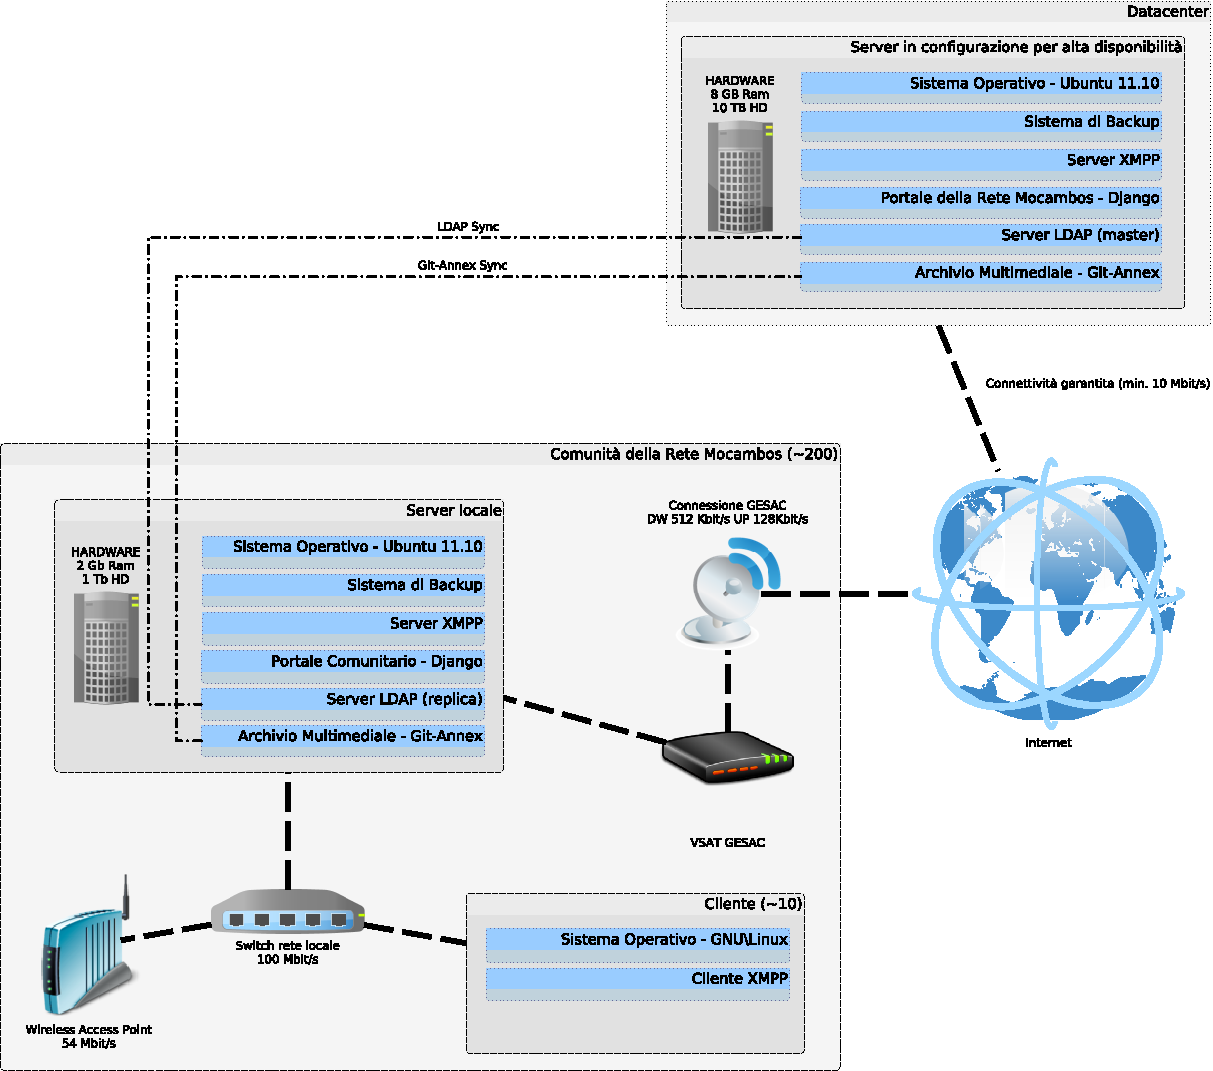
\includegraphics[width=\textwidth]{./Figure/SchemaServer_ReteMocambos-crop.pdf}
  \rule{35em}{0.5pt}
  \caption[Schema dell'infrastruttura della RM]{Schema dell'infrastruttura della RM.}
  \label{fig:SchemaServer_ReteMocambos}
\end{figure}


\section{Archivio multimediale}
L'archivio multimediale locale della comunità è un \emph{repository
  git-annex} (vedi \ref{git-annex}) che viene gestito tramite un
portale comunitario, sia per la pubblicazione che per la
visualizzazione dei contenuti. L'accesso diretto ai dati è comunque
garantito essendo i dati salvati in chiaro sul disco. Inoltre è
possibile interagire con i dati attraverso l'ampio universo di
applicazioni e librerie di \emph{git}. In particolare il prototipo
utilizza la struttura dei metadati di \emph{git} per mantenere traccia
del responsabile della pubblicazione di un contenuto. L'operazione di
\emph{commit} coincide infatti con la pubblicazione di un contenuto, e
il \emph{committer} con l'utente che lo pubblica. I metadati, invece,
relativi al contenuto multimediale in se, quali autore, tipo di
licenza, data di creazione, possono essere memorizzati all'interno del
file seguendo gli standard esistenti come il \emph{Dublin
  Core}\footnote{``Il Dublin Core è un sistema di metadati costituito
  da un nucleo di elementi essenziali ai fini della descrizione di
  qualsiasi materiale digitale accessibile via rete informatica'',
  tratto da Wikipedia:
  \url{http://it.wikipedia.org/wiki/Dublin_Core}.}.

Un aspetto importante per l'archivio multimediale sono le operazioni
di sincronizzazione. Gli strumenti basati su \emph{git} ereditano la
sua natura decentrata e la capacità di comunicare in maniera
trasparente usando una ampia gamma di protocolli. In particolare è
interessante la possibilità di eseguire le sincronizzazioni con
sistemi di archiviazione di massa, caratteristica utile nella fase di
creazione di un nuovo nodo, per cui la prima sincronizzazione via rete
potrebbe richiedere giorni (vedi requisito \ref{Sincronizzazione}). I
trasferimenti comunque avvengono, nel caso di \emph{git-annex},
tramite il protocollo \emph{rsync}\footnote{\emph{rsync} è uno
  programma libero per il trasferimento rapido e incrementale di file,
  disponibile su \url{http://rsync.samba.org/}.}, che gestisce
eventuali interruzioni, evitando costose ritrasmissioni.

\subsection{git-annex}\label{git-annex}
\emph{git-annex}\footnote{\emph{git-annex} è un programma che estende
  le funzionalità di \emph{git} nel gestire file di grandi dimensioni,
  disponibile su \url{http://git-annex.branchable.com}.} permette la
gestione di file con \emph{git}, senza la necessità di aggiungere il
file dentro \emph{git}. Anche se può sembrare paradossale, è utile
quando si ha a che fare con file molto grandi che \emph{git}
attualmente non può gestire facilmente per limitazioni dovute a
memoria, tempo o spazio nel disco.

Anche senza mantenere traccia del contenuto del file, avere la 
possibilità di gestire i file con \emph{git}, di spostarli e cancellarli su un
albero di cartelle versionato, con uso di \emph{branches} e di cloni
distribuiti, sono tutti buoni motivi per usare \emph{git}. E i file allegati
(da cui il nome \emph{git-annex}) possono coesistere nello stesso repository
\emph{git} con i file regolarmente versionati.

\emph{git-annex} trasforma i file allegati in \emph{link}
simbolici, che vengono normalmente versionati da \emph{git}. 

Il contenuto dei file viene mantenuto da \emph{git-annex} in un
archivio chiave/valore distribuito che corrisponde ai cloni di un
dato \emph{repository git}. Praticamente \emph{git-annex} memorizza il
contenuto del file in una sotto-cartella di \verb|.git/annex/|.

La prima volta che un file viene aggiunto a \emph{git-annex}, viene
calcolata una chiave, normalmente facendo un \emph{hash} del suo
contenuto. \emph{git-annex} tuttavia supporta diversi \emph{backend}
che possono produrre vari tipi di chiavi. Il file che viene aggiunto a
\emph{git} non è altro che un \emph{link} simbolico alla chiave
memorizzata in \verb|.git/annex/|. Se il contenuto del file viene
modificato, viene prodotta un'altra chiave, e il \emph{link} viene
cambiato.

Il contenuto del file può essere trasferito da un \emph{repository}
all'altro da \emph{git-annex}, che inoltre mantiene traccia di chi
contiene cosa, permettendo ad esempio di creare una mappa delle copie
disponibili e impostare il numero di copie minime. Queste informazioni
vengono mantenute su un \emph{branch} separato, chiamato
``\emph{git-annex}'', e le operazioni di sincronizzazione non sono
altro che \emph{push} e \emph{pull} tra i vari \emph{repository}.

\emph{git-annex} supporta:
\begin{itemize}
\item localizzazione delle copie (\emph{location tracking})
\item scaricamento selettivo dei contenuti
\item gestione della fiducia dei \emph{repository}
\item gestione del numero di repliche minimo 
\item vari \emph{backend} per le chiavi (SHA\footnote{Secure Hash
    Algoritm, (SHA), è un algoritmo usato in sistemi chiave/valore
    dove le chiavi vengono calcolate tramite una funzione
    crittografica del valore}, WORM\footnote{L'algoritmo WORM
    identifica i file in base a nome, dimensione e data di modifica.})
\item vari \emph{backend} per i contenuti/valori (BUP\footnote{BUP è
    un sistema per il \emph{backup} ad alta efficienza disponibile su:
    \url{https://github.com/apenwarr/bup}.}, rsync, web,
  S3\footnote{Amazon Simple Storage Service, (S3) è un infastruttura
    per la memorizzazione di dati totalmente ridondante, disponibile
    su: \url{aws.amazon.com/}.})
\end{itemize}

\section{Portale Comunitario}
Il portale locale deve dare accesso ai principali servizi locali della
comunità. Per lo sviluppo è stato scelto l'uso di un framework basato
su Python, \emph{Django} (vedi \ref{Django}), che consente
un'integrazione flessibile e avanzata con altri sistemi grazie alle
numerose librerie disponibili quale, ad esempio, quella per
l'autenticazione LDAP.

Per l'installazione del framework e del modello base del prototipo di
portale comunitario è stato creato uno \emph{script} mentre, per
gestire l'archivio multimediale \emph{git-annex} sono stati sviluppati
due moduli per \emph{Django}, che definiscono il modello dei dati e si
prendono cura di aggiungere i contenuti sul \emph{repository}
eseguendo le operazioni di \emph{commit}, \emph{push} e \emph{pull}.

\begin{figure}[htbp]
  \centering
  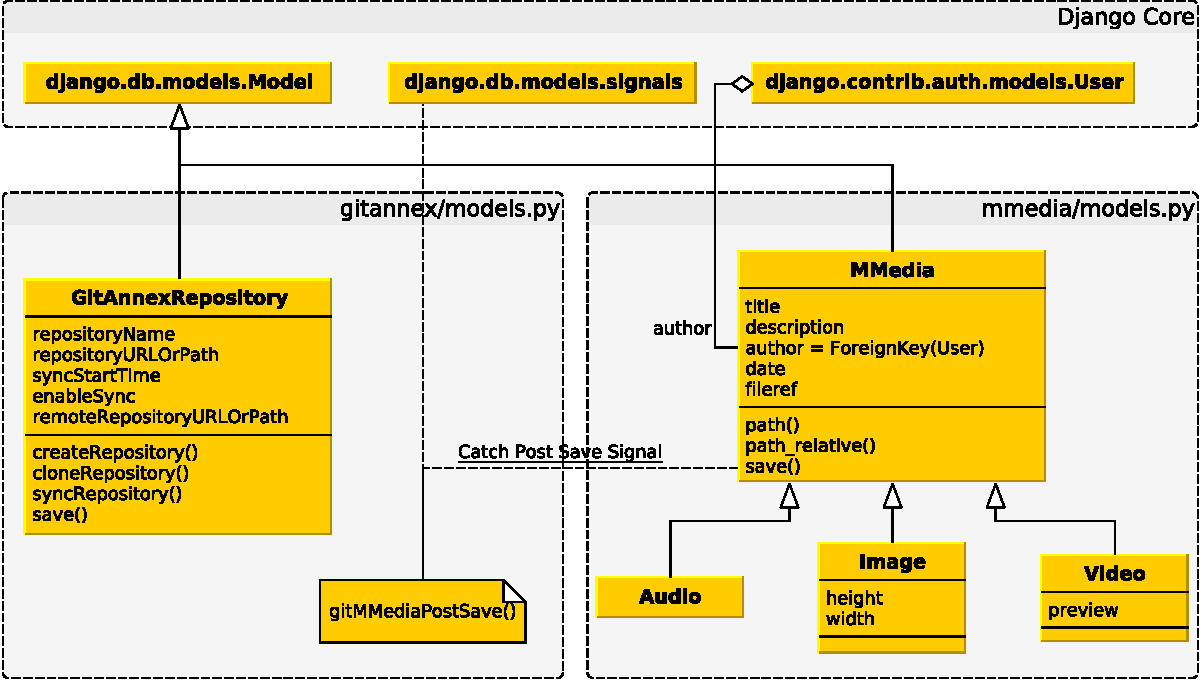
\includegraphics[width=\textwidth]{./Figure/UML_Schema_Django-crop.pdf}
  \rule{35em}{0.5pt}
  \caption[Schema UML dei moduli django]{Schema UML dei moduli django.}
  \label{fig:SchemaUMLDjango}
\end{figure}

\subsection{Mocambos\_Portal\_Local}
\framebox[\textwidth]{\footnotesize Il codice è disponibile su
\url{https://github.com/RedeMocambos/Mocambos_Portal_Local}}

Lo \emph{script bash}, \verb|script/install-django-env.sh|, installa i
pacchetti di sistema necessari, inoltre crea un ambiente virtuale,
usando il programma \emph{virtualenv}\footnote{\emph{Virtualenv} è un
  programma libero per creare ambienti Python isolati disponibile su
  \url{http://www.virtualenv.org}.}, che consente di installare
facilmente versioni specifiche delle librerie e dell'interprete
Python, oltre che di \emph{Django}, senza alterare quelle già presenti
nel sistema. Nella cartella \verb|exemplos/| si trovano invece dei
file di configurazione di esempio, preimpostati per la connessione al
server LDAP della RM (vedi \ref{MocambosLDAP}).


\subsection{Django mmedia}
\framebox[\textwidth]{\footnotesize Il codice è disponibile su
\url{https://github.com/RedeMocambos/mmedia}}

Il modulo \emph{mmedia} implementa il modello dei dati
multimediali con supporto al salvataggio su \emph{repository
  git-annex}.

I modelli, in \emph{Django}, devono essere creati nel file \verb|model.py|,
dove, innanzitutto, definiamo la struttura base della classe
\emph{MMedia}, con gli attributi comuni a tutti gli oggetti
multimediali. Le classi \emph{Audio}, \emph{Image} e \emph{Video},
ereditano dalla classe astratta ``MMedia'', includendo altri attributi
specifici per il tipo di oggetto.

Gli oggetti vengono salvati su \emph{database}, e serializzati su
disco tramite l'\emph{overriding} della funzione \emph{save()}:

\begin{code}
    def save(self, *args, **kwargs):
        logger.debug(type(self))
        serializeTo = os.path.join(settings.MEDIA_ROOT,\
                                   settings.GITANNEX_DIR,\
                                   settings.PORTAL_NAME,\
                                   settings.SERIALIZED_DIR,\
                                   os.path.basename(self.fileref.path)+ '.xml')
        logger.info('>>>> Serialize to: ' + serializeTo)
        out = open(serializeTo, "w")
        XMLSerializer = serializers.get_serializer("xml")
        xml_serializer = XMLSerializer()
        xml_serializer.serialize((self, ), stream=out)
        super(MMedia, self).save(*args, **kwargs)
\end{code}

\subsection{Django gitannex}
\framebox[\textwidth]{\footnotesize Il codice è disponibile su
\url{https://github.com/RedeMocambos/gitannex}}

Il modulo \emph{gitannex} implementa parte del modello dei dati di un
\emph{repository git-annex} in \emph{Django}, aggiungendo gli attributi e le
funzionalità necessarie alla programmazione della sincronizzazione.

\begin{figure}[htbp]
  \centering
  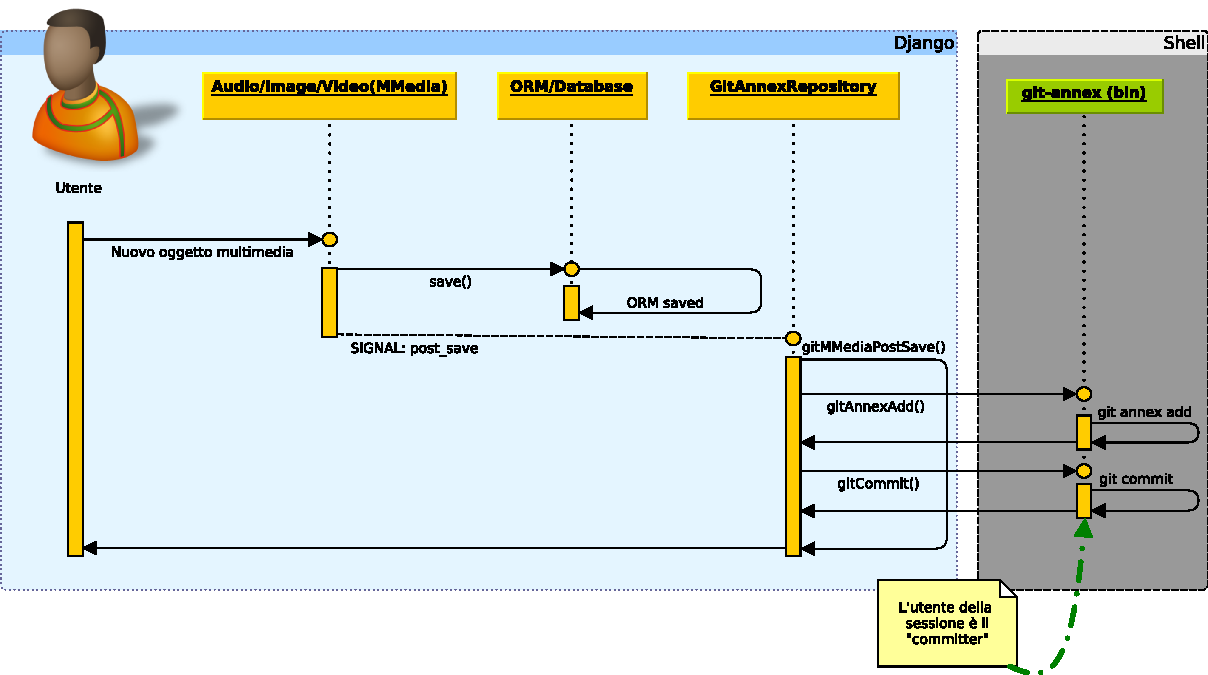
\includegraphics[width=\textwidth]{./Figure/SequenceDiagram_NuovoOggetto-crop.pdf}
  \rule{35em}{0.5pt}
  \caption[Diagramma di sequenza della creazione di un nuovo oggetto
  multimediale]{Diagramma di sequenza della creazione di un nuovo
    oggetto multimediale.}
  \label{fig:SequenceDiagramAdd}
\end{figure}

Seguendo la specifica, viene definito, tramite l'attributo
\emph{syncStartTime}, un orario per l'inizio della sincronizzazione,
che viene lanciata dalla funzione \emph{runScheduledJobs()}. Per
interagire più facilmente con il framework tramite shell è possibile
definire nuovi comandi che devono essere creati nella cartella
\verb|management/commands/|, dove si trova, ad esempio, il comando
\verb|run_scheduled_jobs| che richiama la funzione omonima. In questo
modo è possibile eseguire operazioni programmandole tramite il
\emph{cron}\footnote{``Nei sistemi operativi Unix e Unix-like, il
  comando crontab consente la pianificazione di comandi, ovvero
  consente di registrarli presso il sistema per essere poi mandati in
  esecuzione periodicamente.'', tratto da Wikipedia:
  \url{http://it.wikipedia.org/wiki/Crontab}.} o direttamente da shell
con:
\begin{verbatim}
zumbi@palmares:~$ python manage.py run_scheduled_jobs
\end{verbatim}

\emph{Django} fornisce un sistema di segnali, lanciati in concomitanza di
operazioni quali la \emph{save()} di un oggetto, che possono essere
intercettati altrove dal sistema. Il modulo \emph{gitannex} intercetta
il segnale standard di Django, \emph{post-save} (vedi figura
\ref{fig:SequenceDiagramAdd}), su oggetti che ereditano dalla classe
\emph{MMedia}\footnote{Django non supporta il ``filtraggio'' dei
  segnali lanciati dalle sottoclassi di una data classe, in questo
  caso \emph{MMedia}. A tal fine, è stato usato un trucco reperito in
  rete (vedi il codice nel file \texttt{gitannex/signals.py}).},
tramite la funzione \emph{gitMMediaPostSave()}:

\begin{code}
@receiver_subclasses(post_save, MMedia, ``mmedia_post_save'')
def gitMMediaPostSave(instance, **kwargs):
    logger.debug(instance.mediatype)
    logger.debug(type(instance))
    logger.debug(instance.path_relative())

    path = instance.path_relative().split(os.sep)
    if gitannex_dir in path:
        repositoryName = path[path.index(gitannex_dir) + 1]
        gitAnnexRep = GitAnnexRepository.objects.get(\
                      repositoryName__iexact=repositoryName)
        gitAnnexAdd(os.path.basename(instance.fileref.name),\
                    os.path.dirname(instance.fileref.path))
        gitCommit(instance.title, instance.author.username,\
                  instance.author.email, os.path.dirname(instance.fileref.path))
\end{code}







